\chapter{Introduction}
The last few years personal digital assistants(PDA) or smart-phones have become a gadget we take for granted and need this for our daily activities.  We take notes and make plans during the day, and share this with our friends and family. Our research will take in consideration different methods on how to display these day-to-day notes and how they may affect learning when collaborating on reflection.

For example when a class is on a school-trip and afterwards you want them to write an essay about what they have learned about the destination. If they had the opportunity to take notes they would the ability to go back and read them and use them as a basis for their essay, but let’s say they had the opportunity to use a tool which gives them the ability to collaborate on the notes and being able to review these notes in multiple ways in order to gain the most of them. Being able to see the notes spread out on a map and pinned to the location where they originated will be of great benefit.

Multi-media and multi-representational learning environments are ubiquitous and were so even before the advent of modern educational technology.\cite{Ainsworth1999} By combining three informative ways to display information we give the user an opportunity to view his/her notes or his/her group’s notes in a different way and maybe even put them in perspective. This will help the learners to how to make sense of the information and how to make conscious decision about the use of information. This will give them the opportunity to take a step back and reflect on the information. In order to achieve good results and to further enhance the ability to learn, reflection is needed. These skills are important in both learning with and without technology, but when being supported by technology however, this technology should promote these aspects within learning \cite{Lin1999}.

The goal is to offer technology that not only makes information search and collection efficient, but also support reflection in a collaborative session. Through reflection learning can be achieved and users can collaborate on gathering information for experiences and the ability to reflect over experiences by displaying data in different methods this might enhance the reflection ability and letting the user view data in another way.

\section{Intro}
The Introduction is your thesis in a nutshell. 
Again, the organization can vary, but a
standard introduction includes the following sections:
• Motivation: Brief description of the research domain and the problem that one
wants to address. It should tell the reader why working on this project is worth
doing.
• Context: Very brief description of the context in which the project is done. This
is important if you are conducting your work in the context of a wider project.
• Research questions: What are the questions you are answering with your
project? Normally, you specify a main question and related sub-questions.
Remember that at the end you have to demonstrate you have answered to the
stated questions. It is not uncommon that the questions are changed during the
project, but it is important to be as explicit as possible and as early as possible
with research questions since they help you to focus.
%!TEX root = main.tex
\section{Research Question}

%%%%%%%%%%%%%%%%%%%%%%
% HER ER DET MYE RART?
% Oppdatere?
% The thesis should introduce versiontracking control here, and introduce Github as an example of such a tool. Need to explain why we chose Github(api etc.)
%%%%%%%%%%%%%%%%%%%%%%
\begin{itemize}
	\item How to promote experienced-based learning from reflection based on project artifatcs collected from version-control systems?
	\begin{itemize}
		\item How to scaffold collection of data inorder to promote daily reflection?
		% Dette virker litt langt/det går kanskje inn under et av de andre spm?\item How to give individuals an outline of what they have contributed with as individuals compared to others in a project with multiple contributors for individual reflection?
		\item How to collect daily experiences for use in collaborativ reflection sessions?
		\item How to increase the tendency to reflect on experiences, both individually and as a team? 
		\item How to bring together contributions from multiple users, possibly using different conceptualization of the work process? 
		\item How to support cooperation around these representations?
	\end{itemize}
\end{itemize}
• Research Method: How the research is conducted. In the previous section you
say what you are doing. Here you specify how. The choice of a research method
is strictly connected to the type of questions you want to answer.
%!TEX root = main.tex
%
% ### Research Method
% Where are we getting requirements from?  
% What will guide our design?  
% How will we evaluate the tool?  
%
\section{Research Method}

% Lage et diagram som http://daim.idi.ntnu.no/masteroppgave?id=6231 og Timeline masteroppgaven gjør. Altså hvordan vi har gått frem underveis. Skriv så litt om hver periode, hva vi har gjort etc. Veldig likt timeline bare ikke så mye. Dropp såå alle de subsectionsa under. Går sikkert an å bake inn litt fra de ulike stedene, de bør jo nevnes. F.eks research rigor etc. 

The \emph{Design-Science Research Guidelines} presented in \cite{Esearch2004} the  will serve as the basis of this design-science research. The guidelines were created in order to assist researchers to understand the necessary requirements for effective design-science research. We will also be using the regulative cycle\cite{wieringa}.
\begin{figure}[!htpb]
\label{regulativecycle}
\centering
	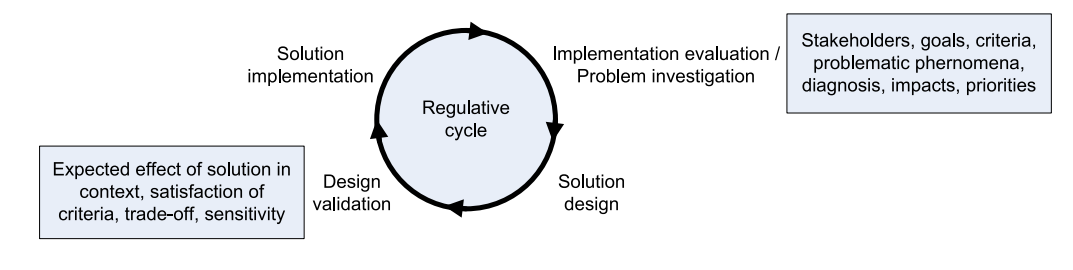
\includegraphics[width=\textwidth]{regulativecycle}
\caption{Regulativecycle development in Design-Science research}
\end{figure}

\subsection{Development steps}
Our researchmodel shows our thesis from initial idea to evaluation and results:

\begin{figure}[!htpb]
\label{researchmodel}
\centering
	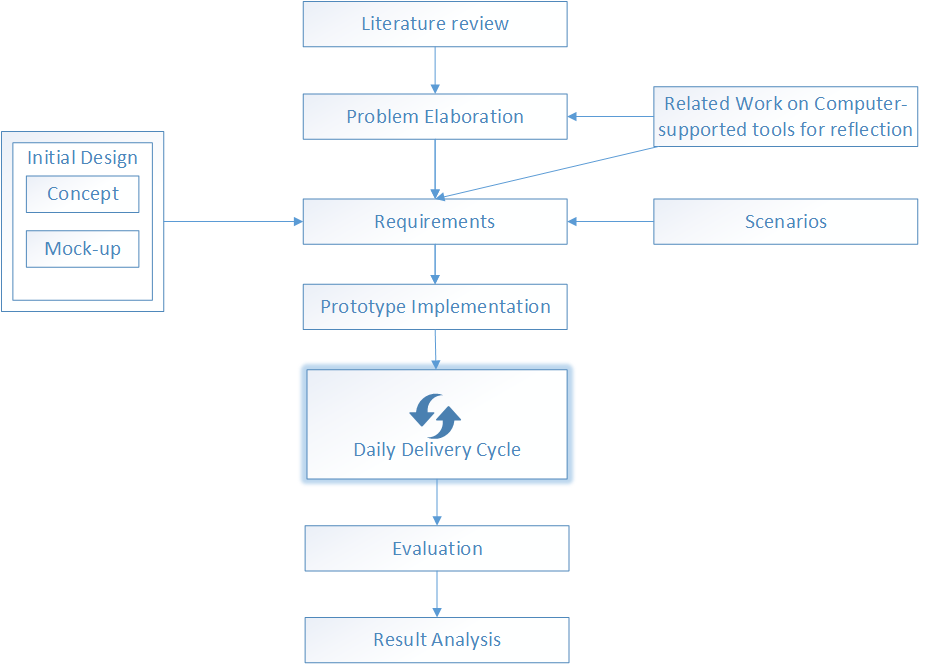
\includegraphics[width=\textwidth]{researchmodel_and_iterationcycle}
\caption{The researchmodel}
\end{figure}

\begin{figure}[!htpb]
\label{iterationprocess}
\centering
	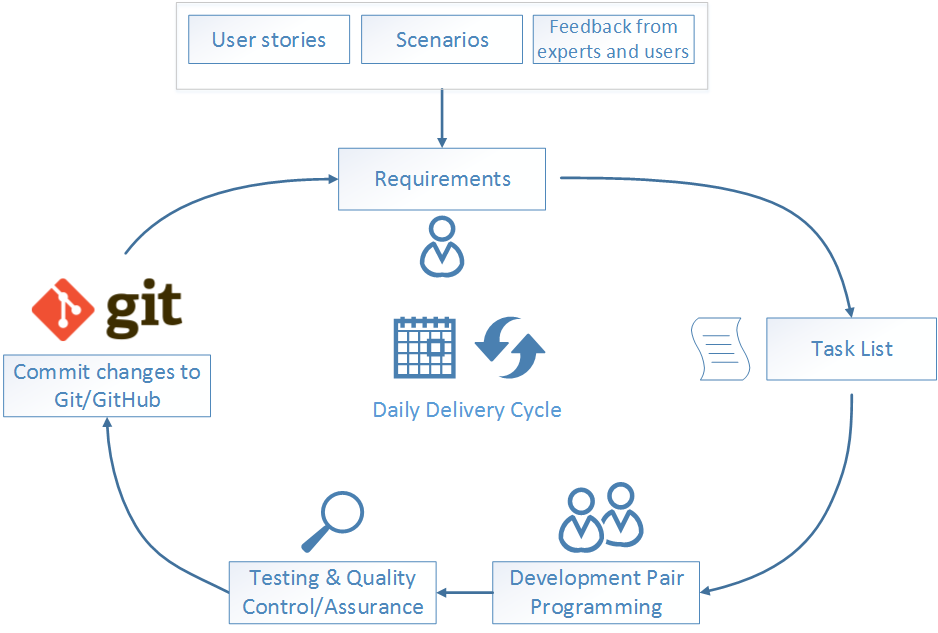
\includegraphics[width=\textwidth]{iterationprocess}
\caption{The daily delivery cycle}
\end{figure}

%Evaluation:
%Core questions described in the toolbox, 9.1:
%Demographic questions, usage of the app, most relevant app-specific questions - choosing the questions that are most important to our thesis. 
%In addition we will use the reflection scale, shown in 9.1.4 both before and after the evaluation period, in order to measure the effect on the tendency to reflect on past
%experiences. Finally we will include the learning outcomes questions and the work behaviour questions, after the evaluation period. 


%Evaluation with the students in IT2901: 
%Students will use the tool for two weeks, daily individual use and as a team after the two week period. 
%For scenario 2 we will require a team of at least 3 people in order to test. 
%The first scenario does not require anything but a github repository. 

\subsection{Design as an artifact}
By definition, the result of design-science research in Information Science is:
\begin{quote}
A purposeful IT artifact created to address an important organizational problem. It must be described effectively, enabling its implementation and application in an appropriate domain.
\end{quote}
\cite{Markus et al. 2002} identified that a developed artifact is only significant if there is questions like: Can it be constructed, can it perform appropriately and is the result important to the information science community. 
We will create a proof of concept prototype tool for promoting experienced-based learning from reflection based on project artifacts collected from version-control systems. Our goal was to create a tool that can discover new capabilites in the domain of reflection and experience-based learning, as well as support the existing capabilities in an efficient way. Evaluating the tool in \emph{real use} situations is necessary in order to discover if the artifact can enhance the reflection process as it is today. 

\subsection{Problem relevance}
We want to explore how the collection and scaffolding of experiences connected to project artifacts can support collaborative reflection sessions. In order to revisit and learn from previous experiences we want to collect and scaffold experiences from users daily. Experiences and memories change over time, so collecting these experiences as quickly as possible is important. The tool will keep a copy of these experiences in order for users to revisit them at a later date, be it individually or in collaborative reflection sessions. These notes will be collected based on tags that are related to the experience being reviewed \cite{Hassan-montero2006}

\subsection{Evaluation}
Table 2 in \cite{Esearch2004} will be used as guidelines for evaluation of our prototype. 
During evaluation we will be using parts of the evaluation toolbox published by MIRROR\footnote{\url{http://www.mirror-project.eu/showroom-a-publications/downloads/finish/5/67}}. This toolbox is a specification of evaluation methodology and research tooling. 

\subsubsection{Observational}
Before and after the user evaluation of the tool, all test-subjects will be given a form with a set of questions to evaluate the application. We will be using core demographic questions, app usage, the most relevant app-specific questions, and also the reflection scale [\ref{reflectionscale}] from the toolbox. The reflection scale assesses participants' general tendency to reflect and the importance they place on reflection. Using this scale, allows us to see whether using the tool prime people to reflect more. Meaning: Does the tool increase the users tendency to reflect on experiences, both individually and as a team. Measuring this before and after using the tool implementation, allows us to measure the expected increase. \\*
Finally we will include the learning outcomes questions and the work behaviour questions, after the evaluation period.  

\subsubsection{Analytical}
We will perform a dynamic analysis on the data collected from server and user feedback. During use the application will provide simple usage-patterns on how the users use the application.
This will also help us in the analysis of the applications performance as well as its usefulness in the reflection and learning domains

\subsubsection{Testing}
During development we will continuously test the tool  to ensure that the user experience is as expected, as a means of quality assurance.
White Box testing will be executed during development of the application with artificial data to ensure that the function is working properly and as specified. 

\subsubsection{Descriptive}
Evaluation proposal with the students in IT2901 - A project course taken by computer science students on the Norwegian University of Science and Technology (NTNU). 
Students that accept to evaluate our tool, will use it for two weeks, with daily individual use and as a team after the two week period. This will allow us to measure the usage of our scenarios. 

Requirements: 
The first scenario does not require anything but a github repository and is doable both for single and for multiples in teams.
For scenario 2 we will require a team of at least 3 people in order to collect enough data. 
We have continuously been using and evaluating the tool ourselves, also a fellow student has been using it for a couple of weeks, so we have some additional evaluation
data also.

\subsection{Research Contributions}
The main goal is to create a proof of concept application that will help users reflect on their past experiences individually and in collaborative reflection sessions by collecting experiences daily and revisiting them at any time. We will analyse the users experience and the evaluation results  in order to draw a conclusion on if multiple representations might help the users to reflect on their past experiences in a collaborative session.

\subsection{Research Rigor}
We will test the tool with a group of experts in the fields relevant and gather data during testing with this group and use this to evaluate the usefulness of the tool. This will serve as a good basis for analysis, triangulate and evaluate to look for relevant research results elsewhere.

\subsection{Design as a redsearch process}
The application will be developed in two main parts, which is central to this research. The first part is development and the second is testing/evaluating the results.

Implementing the application will be developed in development cycles; The first goal will be to develop ideas and a basic mock-up of the application and its design. The second goal will be to implement basic features. Implementation of the individual and collaboration features will then be developed on the basis of feedback from the first cycles. Finally we will focus on integrating all the features into the final system, and create a tool for individual and collaborative reflection use. We will use the tool ourselves during development, as it would be used in a real world environment. In this way we will ensure that all functionality is working as expected, and also identify limitations in the design. 

Finally we will perform the case study evaluation with computer-science students, and the expert review. Evaluating these separately will provide two sets of feedback which we can compare in order to possibly see if any patterns emerge. 

\subsection{Research communication}
The proof of concept application will be available for testing along with a user guide, the whole process will be well documented and our research results will be made available.
Any limitations identified  will be documented along with the research results. 




• Results: a brief description of the results that you are delivering.
• Outline of the report: reading guide briefly describing what each chapter of the
thesis is about.